% \input{fixos/pacotes}
\documentclass[12pt,openright,twoside,a4paper,english,french,spanish,brazil]{abntex2}

\usepackage{cmap}	
\usepackage{lmodern}	
\usepackage[T1]{fontenc}	
\usepackage[utf8]{inputenc}		
\usepackage{lastpage}		
\usepackage{indentfirst}
\usepackage{color}	
\usepackage{graphicx}	
\usepackage{units}
\usepackage[brazilian,hyperpageref]{backref}
\usepackage[alf]{abntex2cite}
\usepackage{bold-extra}
\usepackage{eso-pic}
\input{fixos/comandos}
\usepackage{fixos/customizacoes}

% Dados pessoais
\autor{André de Sousa Costa Filho}
\curso{Engenharia de Software}

% Dados do trabalho
% \titulo{Boas Práticas Na Gerência De Repositórios Git: Um Estudo Sobre Impactos Causados No Desenvolvimento De Software}
\titulo{Título: Subtítulo do Trabalho}
\data{2019}
\palavraChaveUm{Estudo}
\palavraChaveDois{Boas práticas}

% Dados da orientacao
\orientador{Prof. Dr. Renato Coral Sampaio}
\coorientador{Prof. Dr. Carla Rocha Aguiar}

% Dados para a ficha catalográfica
\cdu{02:141:005.6}

% Dados da aprovação do trabalho
\dataDaAprovacao{01 de junho de 2013}
\membroConvidadoUm{Titulação e Nome do Professor Convidado 01}
\membroConvidadoDois{Titulação e Nome do Professor Convidado 02}

% Dados pessoais
\autor{André de Sousa Costa Filho}
\curso{Engenharia de Software}

% Dados do trabalho
% \titulo{Boas Práticas Na Gerência De Repositórios Git: Um Estudo Sobre Impactos Causados No Desenvolvimento De Software}
\titulo{Título: Subtítulo do Trabalho}
\data{2019}
\palavraChaveUm{Estudo}
\palavraChaveDois{Boas práticas}

% Dados da orientacao
\orientador{Prof. Dr. Renato Coral Sampaio}
\coorientador{Prof. Dr. Carla Rocha Aguiar}

% Dados para a ficha catalográfica
\cdu{02:141:005.6}

% Dados da aprovação do trabalho
\dataDaAprovacao{01 de junho de 2013}
\membroConvidadoUm{Titulação e Nome do Professor Convidado 01}
\membroConvidadoDois{Titulação e Nome do Professor Convidado 02}

\input{fixos/setup}

\begin{document}

\frenchspacing 
\imprimircapa
\imprimirfolhaderosto*

\input{fixos/fichaCatalografica}
% \begin{errata}
% Elemento opcional da \citeonline[4.2.1.2]{NBR14724:2011}. \textbf{Caso não 
% deseje uma errata, deixar todo este arquivo em branco}. Exemplo:

% \vspace{\onelineskip}

% FERRIGNO, C. R. A. \textbf{Tratamento de neoplasias ósseas apendiculares com
% reimplantação de enxerto ósseo autólogo autoclavado associado ao plasma
% rico em plaquetas}: estudo crítico na cirurgia de preservação de membro em
% cães. 2011. 128 f. Tese (Livre-Docência) - Faculdade de Medicina Veterinária e
% Zootecnia, Universidade de São Paulo, São Paulo, 2011.

% \begin{table}[htb]
% \center
% \footnotesize
% \begin{tabular}{|p{1.4cm}|p{1cm}|p{3cm}|p{3cm}|}
%   \hline
%   \textbf{Folha} & \textbf{Linha}  & \textbf{Onde se lê}  & \textbf{Leia-se}  \\
%     \hline
%     1 & 10 & auto-conclavo & autoconclavo\\
%   \hline
% \end{tabular}
% \end{table}

% \end{errata}

\input{fixos/folhaDeAprovacao}
\begin{dedicatoria}
   \vspace*{\fill}
   \centering
   \noindent
% 	\textbf{A dedicatória é opcional. Caso não deseje uma, deixar todo este
% 	arquivo em branco}.

   \textit{Este trabalho é dedicado à todos aqueles que me apoiaram e me deram forças durante o decorrer do curso.} \vspace*{\fill}
\end{dedicatoria}

% \begin{agradecimentos}
% A inclusão desta seção de agradecimentos é opcional, portanto, sua inclusão 
% fica a critério do(s) autor(es), que caso deseje(em) fazê-lo deverá(ão) 
% utilizar este espaço, seguindo a formatação de \textit{espaço simples e 
% fonte padrão do texto (sem negritos, aspas ou itálico}.

% \textbf{Caso não deseje utilizar os agradecimentos, deixar toda este arquivo
% em branco}.
% \end{agradecimentos}

% \begin{epigrafe}
%     \vspace*{\fill}
% 	\begin{flushright}
% 		\textbf{A epígrafe é opcional. Caso não deseje uma, deixe todo
% 		este arquivo em branco}.

% 		\textit{``Não vos amoldeis às estruturas deste mundo, \\
% 		mas transformai-vos pela renovação da mente, \\
% 		a fim de distinguir qual é a vontade de Deus: \\
% 		o que é bom, o que Lhe é agradável, o que é perfeito.\\
% 		(Bíblia Sagrada, Romanos 12, 2)}
% 	\end{flushright}
% \end{epigrafe}

\input{editaveis/resumo}
\input{editaveis/abstract}
\input{fixos/listasAutomaticas}
\begin{siglas}
    \item [CLI] Abreviação para \textit{Command Line Interface}, se refere à aplicações executadas na linha de comando.
    \item [UI] Abreviação para \textit{User Interface}.
    \item [FLOSS] Abreviação para \textit{Free Libre Open-Source Software}
\end{siglas}

% \begin{simbolos}
%   \item[$ \Gamma $] Letra grega Gama
%   \item[$ \Lambda $] Lambda
%   \item[$ \zeta $] Letra grega minúscula zeta
%   \item[$ \in $] Pertence
% \end{simbolos}

\input{fixos/indiceAutomatico}

\textual

\part{Introdução e Referêncial Teórico}

\chapter[Introdução]{Introdução}
% \addcontentsline{toc}{chapter}{Introdução}




% tema e contexto
\section{Contexto e introdução teórica}
No cenário de desenvolvimento de software atual, é praticamente obrigatório o uso de ferramentas de versionamento, seja para código, configurações ou para documentação em geral \cite{version_control_git}.

O uso de sistemas e técnicas de versionamento e revisão de versões se tornaram essenciais para o desenvolvimento de software atualmente.
Tais sistemas são encontrados em três diferentes paradigmas: sistemas de versionamento local, sistemas de controle de versão distribuídos - \textit{DVCS} - e sistemas de controle de versão centralizados - \textit{CVCS} \cite{version_control_review}.

Com a contínua expansão da comunidade de software livre, se tornou cada vez mais comum o uso de sistemas DVCS por conta das desvantagens ou impedimentos que os outros paradigmas proporcionavam para o desenvolvimento colaborativo \cite{version_control_review} \cite{version_control_git}.


Inserido neste cenário, o \textit{Git} é uma das ferramentas mais poderosas e utilizadas pelos desenvolvedores de software espalhados mundo afora \cite{git_version_cookbook}. O \textit{Git}, é um software de versionamento de arquivos no formato distribuído criado por Linus Torvalds
% para o desenvolvimento do \textit{kernel Linux} 
e se tornou recentemente a principal tecnologia utilizada para versionamento de repositórios de software \cite{openhub_git_svn}, como demonstra o gráfico de comparação de repositórios tirado do OpenHub (Figura \ref{Fig_comparisson_git}).
De um espaço amostral de 1.296.669 repositórios, aproximadamente 70\% são versionados utilizando o Git, sendo que o Subversion - ou SVN - a segunda maior tecnologia, é utilizado em aproximadamente 25\% dos mesmos.


\begin{figure}[h]
    \centering
    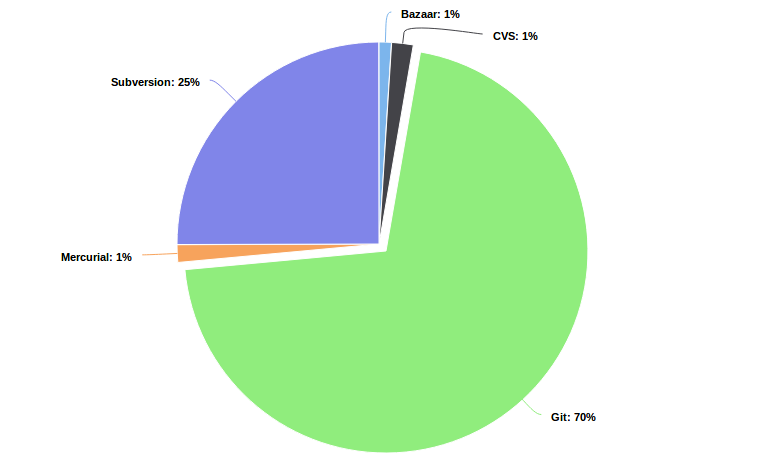
\includegraphics[width=16cm]{figuras/git_svn_comp.png}
    \caption{Comparação de número de repositórios com o Git e outras tecnologias. Fonte: \textit{openhub}}
    \label{Fig_comparisson_git}
\end{figure}

O Git é um software livre que segue a filosofia \textit{FLOSS} e, provavelmente por conta disto, possui uma vasta gama de ferramentas em seu ecossistema a fim de dar suporte ao desenvolvedor.
Além de várias CLIs e UIs voltadas para a ajuda no uso da ferramenta, existem os gerênciadores de repositórios do Git \cite{building_tools_github}. 

Estes gerenciadores são plataformas no qual são submetidas as alterações dos repositórios, sendo as mais utilizadas o \textit{Github}, \textit{GitLab} e \textit{Bitbucket}. Com o uso destas ferramentas, o já presente suporte ao desenvolvimento colaborativo no git se torna mais significante, visto que elas proveêm suporte para diversas formas de organização e distribuição de tarefas para equipes, além de diversas integrações com ferramentas externas. 

% Tal suporte à colaboração não é algo novo, visto que existe desde a concepção do Git por Torvalds \cite{version_control_git}, visto que era um requisito novo e necessário a capacidade de suportar trabalho distribuído e tratar de alterações no mesmo trecho de código. Na realidade atual, tal capacidade é cada vez mais necessária com times de desenvolvimento se tornando cada vez mais distribuídos \cite{developer_survey}.



Tal suporte fez com que as comunidades de software livre utilizassem dessas plataformas para manter seus projetos \textit{open-source} abertos para contribuições externas, de uma forma mais acessível e - em geral - menos burocrática. Considerando o fato de times de desenvolvimento cada vez mais distribuídos estarem se tornando uma realidade progressivamente mais comum \cite{developer_survey}, é possível afirmar que a demanda para plataformas colaborativas é sólida e não deixará de ser significante facilmente.

Com a popularização destas plataformas e do workflow envolvido para a contribuição em softwares livres, começaram a surgir diferentes tipos de documentação, regras e guias voltados à auxiliar desenvolvedores a contribuírem em projetos, mantendo ao mesmo tempo a organização e qualidade dos mesmos.

Seja essa documentação composta dos clássicos  guias de contribuição e \textit{READMEs}, até os novos templates de \textit{pull request}, \textit{issues}, é essêncial que essa documentação exista para guiar novos contribuidores.

Pensando nisso, o Github lançou o dashboard de ferramentas para comunidade em 14 de junho de 2017 \cite{post_github_community_tools} proporcionando recomendações de documentação consideradas como boas práticas para repositórios de software livre, esse dashboard pode ser visto na aba \textit{insights} opção \textit{community}, conforme a figura \ref{Fig_dash_community}.


\begin{figure}[h]
    \centering
    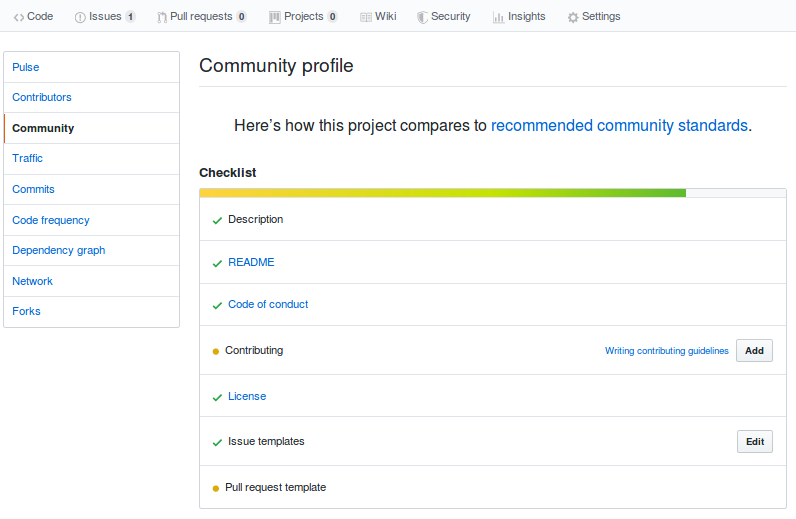
\includegraphics[width=16cm]{figuras/min_dashboard_community.png}
    \caption{Exemplo de dashboard de comunidade no Github}
    \label{Fig_dash_community}
\end{figure}

Segundo essas recomendações, um bom repositório de software livre deve possuir pelo menos os seguintes artefatos \cite{opensource_guidelines_github}:

\begin{itemize}
    \item Descrição do repositório
    \item Arquivo README
    \item Código de conduta
    \item Guia de contribuição
    \item Licença
    \item Template de \textit{issue}
    \item Template de \textit{pull request}
\end{itemize}

Embora aparentemente tenha tomado para si o papel de guia do desenvolvimento \textit{open-source}, por conta de ser a maior e mais usada plataforma de host de repositórios no mundo, não são todos que seguem estas recomendações do Github.
Outras plataformas atualmente não possuem este mesmo recurso de dashboard ou guias como os presentes no Github. Nelas estes são inexistentes ou não se encontram de forma explícita.

Um dos maiores pontos de divergência entre as comunidades de desenvolvimento é o que são consideradas boas práticas e boas políticas de repositório. Existem diversas 'fraturas' acerca do que comunidades de desenvolvimento definem sobre o que é ou não uma boa prática. Por exemplo, o guia de projetos open-source do github define uma checklist de elementos que um bom repositório de software livre deve possuir \cite{opensource_checklist_github}, já a Linux Foundation define uma outra checklist \cite{opensource_checklist_linux_foundation}, possuindo diferentes elementos entre um e outro.

Sejam essas diferenças relacionadas aos commits durante o desenvolvimento de um projeto ou à mínima documentação necessária para um repositório de software livre, a realidade é que existem diversas opiniões - algumas até conflitantes - sobre o assunto.

Ao mesmo tempo que essa ampla gama de opiniões é algo capaz de provocar confusão para o desenvolvedor, ela também provê diferentes experiências e possibilidades de abordagem. Tal flexibilidade é algo notório principalmente considerando a popularidade de metodologias ágeis no cenário de desenvolvimento de software atual, e inclusive a importância que estas mesmas dão para a experimentação e empiricidade em seus processos de desenvolvimento.








\section{O problema}
% o problema
Com tamanha diversidade de padrões, convenções e formatos, é comum que exista bastante inconsistência dentro dos repositórios e projetos de software. Este fato pode ocorrer por vários fatores, sendo o principal deles a adaptação à um contexto diferente de desenvolvimento.

Tal adaptação é custosa de tempo e a adaptabilidade necessária de um desenvolvedor à um contexto de trabalho é um requisito do mercado cada vez mais cobrado. Essa adaptação se torna mais custosa na mesma proporção da quantidade de regras e políticas adotadas na equipe de desenvolvimento.

Uma forma simples de se perceber isso é olhando a árvore de commits - \textit{commit tree} - de um projeto de software. Mesmo com diversas boas práticas de escrita de commit diferentes documentadas, muitos desenvolvedores desconhecem ou não aplicam. Ou no caso dessas boas práticas serem aplicadas e exigidas, caso venha a se ter um novo membro na equipe, a curva de aprendizado dele será impactada.

Uma solução para esses problemas necessitaria de, ao mesmo tempo, ser adaptável para lidar com diferentes padrões e contextos, e ser corretiva além de capaz de guiar a aplicação de boas práticas de acordo com os mesmos.









% objetivos
\section{Objetivos}
Este trabalho tem como objetivos:

\begin{itemize}
    \item Identificar os principais padrões e boas práticas utilizadas em um espaço amostral de repositórios do Github e Gitlab. 
    \item Analisar os padrões e levantar suas características.
    \item Implementar uma ou mais ferramentas capazes de resolver o problema levantado.
\end{itemize}

O espaço amostral citado no primeiro item consistirá dos 5 maiores repositórios de software livre no Github assim como 5 do Gitlab, 5 repositórios de software livre de pequeno a médio porte também presentes em ambas as plataformas e, por fim, 5 repositórios de software livre recentemente criados, totalizando uma amostra de 25 repositórios.


% \chapter{Metodologia de Trabalho}
% \label{metodologia}

% \section{Metodologia Kan Ban}

% % \section{Roadmap}
\chapter{Desenvolvimento}
\label{chapter:desenvolvimento}
% https://www.freecodecamp.org/news/how-to-start-an-open-source-project-in-new-years-945bad8800d7/
% https://www.linuxfoundation.org/resources/open-source-guides/starting-open-source-project/#7
% https://opensource.guide/starting-a-project/#your-pre-launch-checklist
% https://americanexpress.io/on-the-importance-of-commit-messages/
% https://dev.to/maniflames/how-conventional-commits-improved-my-git-skills-1jfk
% https://www.conventionalcommits.org/en/v1.0.0/
% https://medium.com/@andrewhowdencom/anatomy-of-a-good-commit-message-acd9c4490437


% \section{Importância do uso de convenções}
% Não sei como escrever essa parte aqui

\section{O uso do Git}
\label{git_usage_section}

O Git é uma ferramenta bastante poderosa e de fácil uso em sua forma básica, porém seu uso pode se tornar bastante complexo ao se usar funcionalidades mais avançadas. O objetivo desta seção é introduzir elementos e conceitos presentes no restante do trabalho, para garantir um melhor entendimento dos conceitos.

Seja individualmente ou de forma colaborativa, o uso da ferramenta Git gira em torno de três funções fundamentais: \textit{commits}, \textit{branches} e interações com outros repositórios. Cada uma dessas permite, respectivamente, o versionamento, o trabalho em paralelo e o controle de versionamento distribuído.

% o que é um commit
\textit{Commit} é o nome dado para cada versão que o usuário cria com a ferramenta. Um \textit{commit} é formado por: uma hash de identificação criada pelo Git, a identificação do autor, data de criação, uma mensagem associada, a \textit{hash} do \textit{commit} pai e da \textit{branch} a qual o mesmo pertence, além das modificações realizadas. 

Essas versões podem ser acessadas à qualquer momento pelo desenvolvedor, por meio da hash identificadora de cada \textit{commit}. O Git é capaz de listar todas as versões que se possui até aquele momento a partir do commando \textbf{git log} como pode ser visto na Figura \ref{fig:commit_example}.

Nessa exibição, as alterações realizadas - chamadas dentro da ferramenta de \textit{diff} - são ocultadas para o usuário, assim sendo, se torna perceptível a importância da mensagem presente em um \textit{commit}. Mais adiante, boas práticas e conceitos relacionados ao \textit{commit} serão melhor abordados na Seção \ref{section:commit}. % \cite{mastering_git}

\begin{figure}[h]
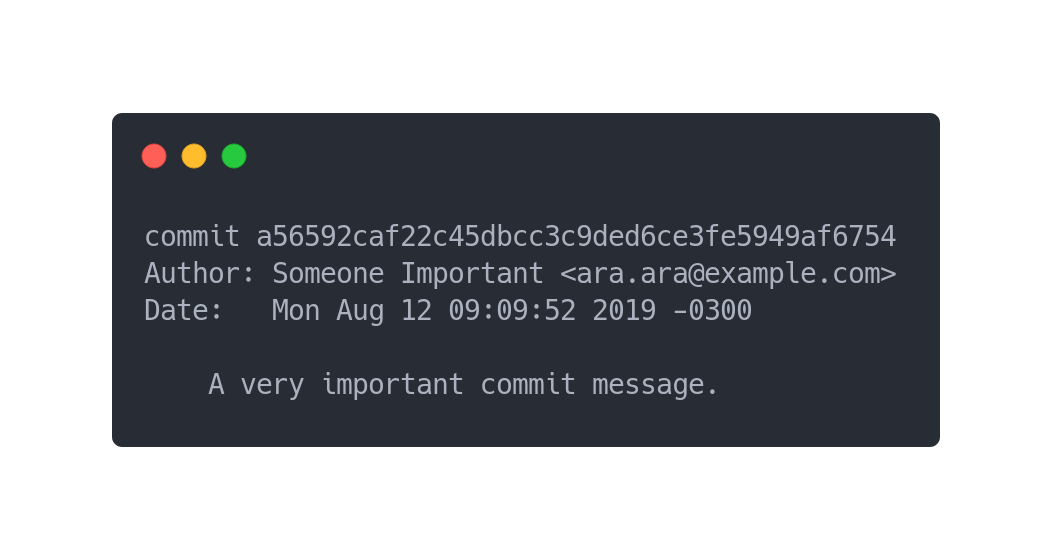
\includegraphics[width=12cm]{figuras/carbon.png}
\centering
\label{fig:commit_example}
\caption{Exemplo de um commit como visto em um \textbf{git log}.}
\end{figure}

% o que são branches
Um outro conceito fundamental do Git são as \textit{branches}. Uma \textit{branch} funciona como uma lista ligada de \textit{commits}, já que cada um possui a referência do seu anterior. Por padrão, o Git proporciona ao usuário uma \textit{branch} padrão, chamada \textit{master}. Essa branch é criada junto ao primeiro \textit{commit} de um repositório. O uso de \textit{branches} permite o desenvolvimento paralelo de diversas atividades dentro de um repositório de trabalho.

Relacionado as \textit{branches}, está a árvore de \textit{commits}. Ela é uma forma de visualizar as \textit{branches} e seus respectivos \textit{commits}. Uma representação de uma árvore de \textit{commits} - ou \textit{commit tree} - pode ser vista na Figura \ref{fig:git_tree}.  A utilização de \textit{branches} é um dos pilares principais que suportam a capacidade do Git de permitir trabalho simultâneo e colaborativo, visto que cada colaborador pode realizar alterações em sua \textit{branch} sem interferir com o trabalho de outro.

% http://jsfiddle.net/fracz/q76vj8ow/

\textit{Branches} também são extremamente importantes para uma boa organização do repositório, geralmente possuindo em repositórios de software sua própria política a ser seguida pelos contribuidores.

\begin{figure}[b]
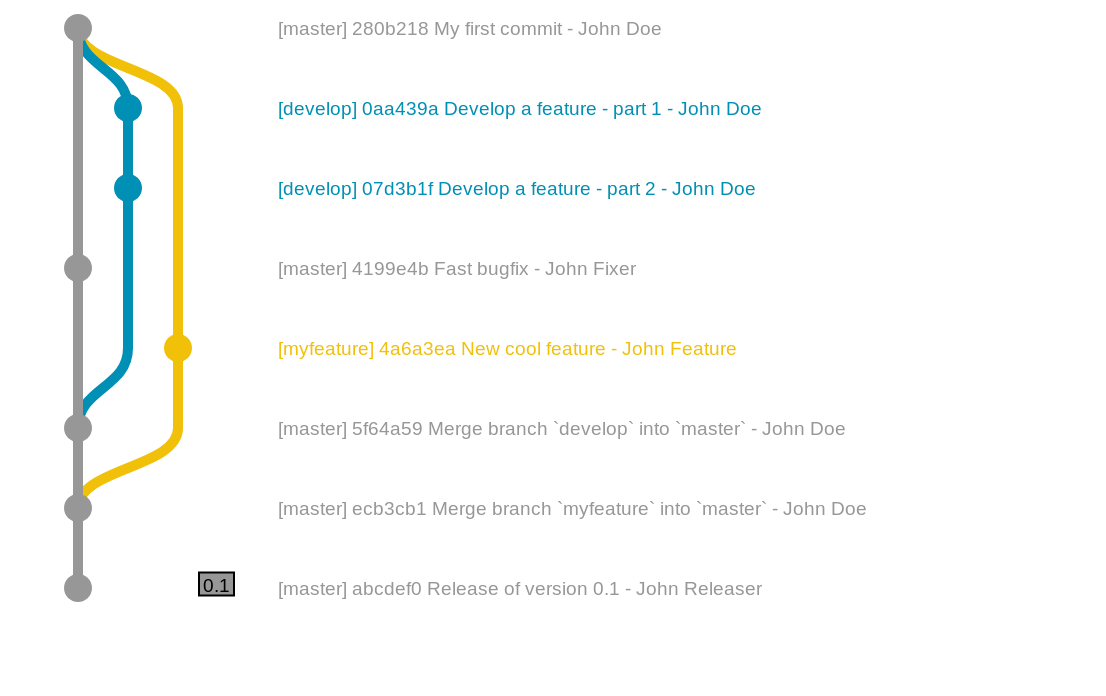
\includegraphics[width=12cm]{figuras/gittree.png}
\centering
\label{fig:git_tree}
\caption{Exemplo de uma \textit{git tree} com 3 \textit{branches}. Cada ponto representa um \textit{commit} e cada cor representa uma \textit{branch} diferente. Fonte: http://jsfiddle.net/fracz/q76vj8ow/}
\end{figure}


% como se dá a interação com outros repositórios
Por se tratar de um sistema de versionamento distribuído, o Git possui ferramentas de gerenciamento de repositórios, permitindo que o usuário gerencie as mudanças realizadas no seu repositório local e as submeta para o repositório em um servidor e vice-versa. O Git realiza tais ações por meio da mesclagem de \textit{branches}. Essa mesclagem pode ocorrer entre \textit{branches} presentes no repositório local e entre \textit{branches} localizadas no repositório local e na nuvem.

% O Git é uma ferramenta bastante poderosa e de fácil uso em sua forma básica, porém seu uso pode se tornar bastante complexo ao se usar funcionalidades mais avançadas. O objetivo desta seção é introduzir elementos e conceitos presentes no restante do trabalho, para garantir um melhor entendimento dos conceitos.

% 
% 
% 
% 
% 
% 
% 
\newpage
\section{O \textit{commit}}
\label{section:commit}

\subsection{O uso de \textit{commits} como parte de documentação de software}
% documentação de software
É algo já estabelecido na área de engenharia e desenvolvimento de software a importância da documentação. Seja em forma de documentos, tutoriais, testes e diagramas ou seja na forma de artefatos menos formais, como \textit{issues} e discussões a cerca de código \cite{importance_of_software_documentation}.

Segundo Sommerville, a documentação de um produto de software faz parte do que é denominado software \cite{sommerville_o_que_eh_software}, portanto artefatos presentes no processo de desenvolvimento de software com o intuito de informar ou ajudar desenvolvedores ou colaboradores externos fazem parte da documentação do software por consequência.

% o que sao commits no git
Durante o processo de desenvolvimento de software, especialmente considerando a cultura de colaboração presente atualmente, desenvolvedores somos constantemente incentivados a versionar o código que trabalhamos.
A importância de tal prática é deveras considerável, visto que um bom gerenciamento de versões permite um controle maior nas alterações submetidas.
% Seja para facilitar a integração com as alterações de um outro colaborador, ou para sinalizar a inserção de uma nova funcionalidade, a importância de se versionar não é algo questionável.

Como dito préviamente, no cenário atual de desenvolvimento de software a principal ferramenta de versionamento utilizada é o Git. O sistema de versionamento do Git ocorre a partir de \textit{commits}.

% como commits se encaixam como documentação


\subsection{Principais boas práticas de \textit{commit}}

% importancia de bons commits

% o que é visto como boas práticas de commit pela comunidade

\subsection{Principais convenções de \textit{commit}}
\subsubsection{Convenção angular}

% referencias

% principais pontos da convenção

% exemplos de uso

% the good and the bad

\subsubsection{Convenção karma}

% referencias

% principais pontos da convenção

% exemplos de uso

% the good and the bad

\subsubsection{Convenção changelog}

% referencias

% principais pontos da convenção

% exemplos de uso

% the good and the bad

\subsubsection{Convenção symphony cmf}

% referencias

% principais pontos da convenção

% exemplos de uso

% the good and the bad


\subsection{Ferramentas de auxílio à escrita de \textit{commit} seguindo convenções}
\subsubsection{Commitzen}
\subsubsection{Commit Helper} % coloco aqui mesmo?




\newpage
\section{Convenções de repositórios de software}

\subsection{O \textit{git flow}}

\subsection{O \textit{semantic versioning}}

\subsection{Documentação padrão}



\newpage
\section{Proposta de trabalho}
% \input{editaveis/aspectosgerais}
% \input{editaveis/consideracoes}
% \input{editaveis/textoepostexto}
% \input{editaveis/elementosdotexto}
% \input{editaveis/elementosdopostexto}

\bookmarksetup{startatroot} 

\postextual

\bibliography{bibliografia} 
% \begin{apendicesenv}

% \partapendices

% \chapter{Primeiro Apêndice}

% Texto do primeiro apêndice.

% \chapter{Segundo Apêndice}

% Texto do segundo apêndice.

% \end{apendicesenv}

% \begin{anexosenv}

% \partanexos

% \chapter{Primeiro Anexo}

% Texto do primeiro anexo.

% \chapter{Segundo Anexo}

% Texto do segundo anexo.

% \end{anexosenv}


\printindex

\end{document}

